\documentclass[a4paper,11pt,fleqn,twoside,openright]{memoir} % Brug openright hvis chapters skal starte p� h�jresider; openany, oneside
%\usepackage{fancyhdr}%mega nemt sidehoved/fod%virker ikke med memoir �benbart
%%%% PACKAGES %%%%

%\usepackage[T1]{fontenc}
%\usepackage{pgfplots}%Ting til grafer (sat ind december 2012)
%\pgfplotsset{
%  compat=newest,
%  xlabel near ticks,
%  ylabel near ticks
%} Ting til grafer (sat ind december 2012)

\usepackage[english]{babel}							% Dansk sporg, f.eks. tabel, figur og kapitel
%\usepackage{pst-plot,pst-node}
%\usepackage[pdf]{pstricks} % G�r det muligt at tegne vektor grafik.
\usepackage{auto-pst-pdf,pstricks-add}
% �� Overs�ttelse og tegns�tning �� %
%\usepackage[ansinew]{inputenc}					% G�r det muligt at bruge �, � og � i sine .tex-filer

%\usepackage[T1]{fontenc}								% Hj�lper med orddeling ved �, � og �. S�tter fontene til at v�re ps-fonte, i stedet for bmp					

% �� FONTS �� % LaTeX er fanme ringe til skrifttyper!
%\usepackage{txfonts}									% konflikter med et eller andet.. giver i hvert fald fejl
\usepackage{mathptmx}								% times (den vi normalt bruger - bare ingen fed mat skrift)
%\usepackage{fourier}									% s�dan lidt middle ground mellem times og pazo (har heller ikke mathbf)
%\usepackage{mathpazo}								% Har fed tekst i matematik (minus mathbf), grim almindelig skrift
%\usepackage{mtpro2}									% f�lger ikke med som standard, men hvis nogen kan installere det skal de da v�re velkomne

\usepackage{latexsym}										% LaTeX symboler
\usepackage{xcolor,ragged2e,fix-cm}			% Justering af elementer
\usepackage{pdfpages}										% G�r det muligt at inkludere pdf-dokumenter med kommandoen \includepdf[pages={x-y}]{fil.pdf}	
\pretolerance=2500 											% G�r det muligt at justre afstanden med ord (h�jt tal, mindre orddeling og mere space mellem ord)
\usepackage{ulem}                       % Gennemstregning af ord med koden \sout{}
\usepackage{fixltx2e}										% Retter forskellige bugs i LaTeX-kernen
\usepackage[shortlabels]{enumitem}			% Muligg�r enkelt konfiguration af lister
\usepackage{alltt}											% Bruges af highlighting (matlab kode)
%\usepackage{Lastpage}

%Matlab kode hightlighting
 \definecolor{string}{rgb}{0.7,0.0,0.0}
    \definecolor{comment}{rgb}{0.13,0.54,0.13}
    \definecolor{keyword}{rgb}{0.0,0.0,1.0}
											
%Include cpp coding in text
\usepackage{listings}
\usepackage{color}

\definecolor{dkgreen}{rgb}{0,0.6,0}
\definecolor{gray}{rgb}{0.5,0.5,0.5}
\definecolor{mauve}{rgb}{0.58,0,0.82}

\lstset{frame=tb,
  language=C++,  
  aboveskip=3mm,
  belowskip=3mm,
  showstringspaces=false,
  columns=flexible,
  basicstyle={\small\ttfamily},
  numbers=none,
  numberstyle=\tiny\color{gray},
  keywordstyle=\color{blue},
  commentstyle=\color{dkgreen},
  stringstyle=\color{mauve},
  breaklines=true,
  breakatwhitespace=true,
  tabsize=3
}											
																			
% �� Figurer og tabeller � floats  �� %
\usepackage{flafter}										% S�rger for at dine floats ikke optr�der i teksten f�r de er sat ind.
\usepackage{multirow}                		% Fletning af r�kker
\usepackage{hhline}                   	% Dobbelte horisontale linier
\usepackage{multicol}         	        % Fletning af kolonner
\usepackage{colortbl} 									% Mulig�re farver i tabeller
\usepackage{rotating}										% Muligg�r rotation af tekst i tabeller med \begin{sideways}...\end{sideways}
\usepackage{wrapfig}										% Inds�ttelse af figurer omsv�bt af tekst. \begin{wrapfigure}{Placering}{St�rrelse}
\usepackage{graphicx} 									% Pakke til jpeg/png billeder
%\pdfoptionpdfminorversion=6%							% Muligg�r inkludering af pdf dokumenter, af version 1.6 og h�jere
\usepackage{tabularx} %Muligg�r at man kan str�kke en tabel-kolonne til �nsket l�ngde
\newsubfloat{figure}
\usepackage{epstopdf}

% �� Matematiske formler og maskinkode ��
\usepackage{amsmath, amssymb} 	% Bedre matematik og ekstra fonte 
\usepackage{textcomp}                 	% Adgang til tekstsymboler
\usepackage{mathtools}									% Udvidelse af amsmath-pakken. 
\usepackage{eso-pic}										% Tilf�j billedekommandoer p� hver side
\usepackage{lipsum}											% Dummy text \lipsum[..]



% �� Referencer, bibtex og url'er �� %
\usepackage{url}												% Til at s�tte urler op med. Virker sammen med hyperref
\usepackage[english]{varioref}						% Giver flere bedre mulighed for at lave krydshenvisninger
%\usepackage{natbib}											% Litteraturliste med forfatter-�r og nummerede referencer
%\usepackage{cite} 												% G�r det muligt at nummere kilder
\usepackage{xr}													% Referencer til eksternt dokument med \externaldocument{<NAVN>}
\usepackage{nomencl}										% Pakke til at danne nomenklaturliste
\makenomenclature												% Nomenklaturliste


% �� Floats �� %
\let\newfloat\relax 										% Memoir har allerede defineret denne, men det g�r float pakken ogs�
\usepackage{float}

\usepackage[footnote,draft,english,silent,nomargin]{fixme}		% Inds�t rettelser og lignende med \fixme{...} Med final i stedet for draft, udl�ses en error 																															for hver fixme, der ikke er slettet, n�r rapporten bygges.

%%%% CUSTOM SETTINGS %%%%

% �� Marginer �� %
\setlrmarginsandblock{3.5cm}{2.5cm}{*}	% \setlrmarginsandblock{Indbinding}{Kant}{Ratio}
\setulmarginsandblock{2.5cm}{3.0cm}{*}	% \setulmarginsandblock{Top}{Bund}{Ratio}
\checkandfixthelayout 									% Laver forskellige beregninger og s�tter de almindelige l�ngder op til brug ikke memoir pakker

%	�� Afsnitsformatering �� %
\setlength{\parindent}{0mm}           	% St�rrelse af indryk
\setlength{\parskip}{4mm}          			% Afstand mellem afsnit ved brug af double Enter
\linespread{1,1}												% Linie afstand

% �� Litteraturlisten �� %
%\bibpunct[,]{[}{]}{;}{a}{,}{,} 					% Definerer de 6 parametre ved Harvard henvisning (bl.a. parantestype og seperatortegn)
%\bibliographystyle{bibtex/harvard}			% Udseende af litteraturlisten. Ligner dk-apali - mvh Klein

% �� Indholdsfortegnelse �� %
\setsecnumdepth{subsection}		 					% Dybden af nummerede overkrifter (part/chapter/section/subsection)
\maxsecnumdepth{subsection}							% �ndring af dokumentklassens gr�nse for nummereringsdybde
\settocdepth{subsection} 								% Dybden af indholdsfortegnelsen

% �� Lister �� %
\setlist{
  topsep=-1ex,														% Vertikal afstand mellem tekst og listen
  itemsep=-1ex,													% Vertikal afstand mellem items
  partopsep=-0ex,
  parsep=1ex
} 

% �� Visuelle referencer �� %
\usepackage[colorlinks]{hyperref}			 	% Giver mulighed for at ens referencer bliver til klikbare hyperlinks. .. [colorlinks]{..}
\hypersetup{pdfborder = 0}							% Fjerner ramme omkring links i fx indholsfotegnelsen og ved kildehenvisninger ��
\hypersetup{														%	Ops�tning af farvede hyperlinks
    colorlinks = false,
    linkcolor = black,
    anchorcolor = black,
    citecolor = black
}

\definecolor{gray}{gray}{0.80}					% Definerer farven gr�

% �� Ops�tning af figur- og tabeltekst �� %
 	\captionnamefont{
 		\small\bfseries\itshape}						% Ops�tning af tekstdelen ("Figur" eller "Tabel")
  \captiontitlefont{\small}							% Ops�tning af nummerering
  \captiondelim{. }											% Seperator mellem nummerering og figurtekst
  \hangcaption													%	Venstrejusterer flere-liniers figurtekst under hinanden
  \captionwidth{\linewidth}							% Bredden af figurteksten
	\setlength{\belowcaptionskip}{-15pt}		% Afstand under figurteksten
		
% �� Navngivning �� %
\addto\captionsenglish{
	\renewcommand\appendixname{Appendix}
	\renewcommand\contentsname{Table of Contents}	
	\renewcommand\appendixpagename{Appendix}
	\renewcommand\cftchaptername{\chaptername~}				% Skriver "Kapitel" foran kapitlerne i indholdsfortegnelsen
	\renewcommand\cftappendixname{\appendixname~}			% Skriver "Bilag" foran bilagene i indholdsfortegnelsen
	\renewcommand\appendixtocname{Appendix}
}

% �� Kapiteludssende �� %


\definecolor{numbercolor}{gray}{0.7}			% Definerer en farve til brug til kapiteludseende
\newif\ifchapternonum

\makechapterstyle{jenor}{									% Definerer kapiteludseende -->
  \renewcommand\printchaptername{}
  \renewcommand\printchapternum{}
  \renewcommand\printchapternonum{\chapternonumtrue}
  \renewcommand\chaptitlefont{\fontfamily{pbk}\fontseries{db}\fontshape{n}\fontsize{25}{35}\selectfont\raggedleft}
  \renewcommand\chapnumfont{\fontfamily{pbk}\fontseries{m}\fontshape{n}\fontsize{1in}{0in}\selectfont\color{numbercolor}}
  \renewcommand\printchaptertitle[1]{%
    \noindent
    \ifchapternonum
    \begin{tabularx}{\textwidth}{X}
    {\let\\\newline\chaptitlefont ##1\par} 
    \end{tabularx}
    \par\vskip-2.5mm\hrule
    \else
    \begin{tabularx}{\textwidth}{Xl}
    {\parbox[b]{\linewidth}{\chaptitlefont ##1}} & \raisebox{-15pt}{\chapnumfont \thechapter}
    \end{tabularx}
    \par\vskip2mm\hrule
    \fi
  }
}																						% <--

%BLUEBOX KAPITEL
\newsavebox{\ChpNumBox}
\definecolor{ChapBlue}{rgb}{1,0,0} % !!
\makeatletter
\newcommand*{\thickhrulefill}{%
\leavevmode\leaders\hrule height 1\p@ \hfill \kern \z@}
\newcommand*\BuildChpNum[2]{%
\begin{tabular}[t]{@{}c@{}}
\makebox[0pt][c]{#1\strut} \\[.5ex]
\colorbox{ChapBlue}{%
\rule[-10em]{0pt}{0pt}%
\rule{1ex}{0pt}\color{black}#2\strut
\rule{1ex}{0pt}}%
\end{tabular}}
\makechapterstyle{BlueBox}{%
\renewcommand{\chapnamefont}{\large\scshape}
\renewcommand{\chapnumfont}{\Huge\bfseries} 		
\renewcommand{\chaptitlefont}{\raggedright\Huge\scshape} % \bfseries
\setlength{\beforechapskip}{10pt}	%DEFAULT:20pt
\setlength{\midchapskip}{20pt}	%DEFAULT:26pt
\setlength{\afterchapskip}{15pt}	%DEFAULT:40pt !!
\renewcommand{\printchaptername}{}
\renewcommand{\chapternamenum}{}
\renewcommand{\printchapternum}{%
\sbox{\ChpNumBox}{%
\BuildChpNum{\chapnamefont\@chapapp}%
{\chapnumfont\thechapter}}}
\renewcommand{\printchapternonum}{%
\sbox{\ChpNumBox}{%
\BuildChpNum{\chapnamefont\vphantom{\@chapapp}}%
{\chapnumfont\hphantom{\thechapter}}}}
\renewcommand{\afterchapternum}{}
\renewcommand{\printchaptertitle}[1]{%
\usebox{\ChpNumBox}\hfill
\parbox[t]{\hsize-\wd\ChpNumBox-1em}{%
\vspace{\midchapskip}%
\thickhrulefill\par
\chaptitlefont ##1\par}}%
}


% Valg af kapiteludseende - dette kan udskiftes efter �nske
%\chapterstyle{madsen}	%P1-style		
\chapterstyle{BlueBox}									

% �� Sidehoved �� %

\makepagestyle{custom}		% Definerer sidehoved og sidefod - kan modificeres efter �nske -->
\makepsmarks{custom}{																						
\def\chaptermark##1{\markboth{\itshape\thechapter. ##1}{}}		% Henter kapitlet den p�g�ldende side h�rer under med kommandoen \leftmark. \itshape g�r teksten kursiv
\def\sectionmark##1{\markright{\thesection. ##1}{}}					% Henter afsnittet den p�g�ldende side h�rer under med kommandoen \rightmark
}																														% Sidetallet skrives med kommandoen \thepage	
\makeevenhead{custom}{Computational Physics}{}{\leftmark}							% Definerer lige siders sidehoved efter modellen \makeevenhead{Navn}{Venstre}{Center}{H�jre}
\makeoddhead{custom}{\rightmark}{}{University of Oslo}			% Definerer ulige siders sidehoved efter modellen \makeoddhead{Navn}{Venstre}{Center}{H�jre}
\makeevenfoot{custom}{\thepage}{}{}													% Definerer lige siders sidefod efter modellen \makeevenfoot{Navn}{Venstre}{Center}{H�jre}
\makeoddfoot{custom}{}{}{\thepage}														% Definerer ulige siders sidefod efter modellen \makeoddfoot{Navn}{Venstre}{Center}{H�jre}		
\makeheadrule{custom}{\textwidth}{0.5pt}											% Tilf�jer en streg under sidehovedets indhold
\makefootrule{custom}{\textwidth}{0.5pt}{1mm}								% Tilf�jer en streg under sidefodens indhold

\copypagestyle{nychapter}{custom}														% F�lgende linier s�rger for, at sidefoden bibeholdes p� kapitlets f�rste side
\makeoddhead{nychapter}{}{}{}
\makeevenhead{nychapter}{}{}{}
\makeheadrule{nychapter}{\textwidth}{0pt}
\aliaspagestyle{chapter}{nychapter}													% <--

\pagestyle{custom} %normalt plain% Valg af sidehoved og sidefod
\usepackage[left=2.4cm, right=2.4cm, top=3cm, bottom=3cm]{geometry}	%Overrider tidliger marginer - men det er lidt mere simpelt.

%%%% CUSTOM COMMANDS %%%%
%referencer
\newcommand{\figref}[1]{Fig.~\ref{#1}}
\newcommand{\tabref}[1]{Tab.~\ref{#1}}	
\newcommand{\matref}[1]{Eq.~\eqref{#1}}
\newcommand{\chapref}[1]{Chap.~\ref{#1}}
\newcommand{\secref}[1]{Sec.~\ref{#1}}
\newcommand{\subsecref}[1]{Subsec.~\ref{#1}}
\newcommand{\appref}[1]{App.~\ref{#1}}
\newcommand{\citer}[1]{\citep[Se][]{#1}}
\newcommand{\citerk}[2][]{\citep[Se][kap.~#1]{#2}}
\newcommand{\citers}[2][]{\citep[Se][s.~#1]{#2}}


% �� Billede hack �� %
\newcommand{\figur}[4]{
		\begin{figure}[H] \centering
			\includegraphics[width=#1\textwidth]{billeder/#2}
			\caption{#3}\label{#4}
		\end{figure} 
		}
		
% �� Specielle tegn �� %
\newcommand{\grader}{\ensuremath{^{\circ}\text{C}}}
\newcommand{\gr}{\ensuremath{^{\circ}}}
\newcommand{\g}{\cdot}


% �� Promille-hack (\promille) �� %
\newcommand{\promille}{%
  \relax\ifmmode\promillezeichen
        \else\leavevmode\(\mathsurround=0pt\promillezeichen\)\fi}
\newcommand{\promillezeichen}{%
  \kern-.05em%
  \raise.5ex\hbox{\the\scriptfont0 0}%
  \kern-.15em/\kern-.15em%
  \lower.25ex\hbox{\the\scriptfont0 00}}

\newcommand{\HRule}{\rule{\linewidth}{0.5mm}}

% �� CUSTOM MATEMATIK/FYSIK-TING ��
\renewcommand{\v}[1]{\ensuremath{\mbox{\textbf{#1}}}} % for vectors
\newcommand{\gv}[1]{\ensuremath{\mbox{\boldmath$ \vec{#1}  $}}} 
% for vectors of Greek letters
\newcommand{\uv}[1]{\ensuremath{\mbox{\boldmath$ \hat{#1}  $}}}  % for unit vector
\newcommand{\abs}[1]{\left| #1 \right|} % for absolute value
\newcommand{\avg}[1]{\left< #1 \right>} % for average
\let\underdot=\d % rename builtin command \d{} to \underdot{}
\renewcommand{\d}[2]{\frac{d #1}{d #2}} % for derivatives
\newcommand{\dd}[2]{\frac{d^2 #1}{d #2^2}} % for double derivatives
\newcommand{\pd}[2]{\frac{\partial #1}{\partial #2}} 
% for partial derivatives
\newcommand{\pdd}[2]{\frac{\partial^2 #1}{\partial #2^2}} 
% for double partial derivatives
\newcommand{\pdc}[3]{\left( \frac{\partial #1}{\partial #2}
 \right)_{#3}} % for thermodynamic partial derivatives
\newcommand{\ket}[1]{\left| #1 \right>} % for Dirac bras
\newcommand{\bra}[1]{\left< #1 \right|} % for Dirac kets
\newcommand{\braket}[2]{\left< #1 \vphantom{#2} \right|
 \left. #2 \vphantom{#1} \right>} % for Dirac brackets
\newcommand{\matrixel}[3]{\left< #1 \vphantom{#2#3} \right|
 #2 \left| #3 \vphantom{#1#2} \right>} % for Dirac matrix elements
\newcommand{\grad}[1]{\gv{\nabla} #1} % for gradient
\let\divsymb=\div % rename builtin command \div to \divsymb
\renewcommand{\div}[1]{\gv{\nabla} \cdot #1} % for divergence
\newcommand{\curl}[1]{\gv{\nabla} \times #1} % for curl
\let\baraccent=\= % rename builtin command \= to \baraccent
\renewcommand{\=}[1]{\stackrel{#1}{=}} % for putting numbers above =
\renewcommand\Re{\operatorname{Re}}
\renewcommand\Im{\operatorname{Im}}
\newcommand{\comp}[1]{\widetilde{#1}}
\newcommand{\unit}[1]{\ensuremath{\, \mathrm{#1}}}

\newcommand{\eqvref}[1]{(\ref{#1}) p� side \pageref{#1}}

\newcommand{\forsog}[1]{\underline{#1}}

\newcommand{\superscript}[1]{\ensuremath{^{\textrm{#1}}}}
\newcommand{\subscript}[1]{\ensuremath{_{\textrm{#1}}}}


%%%% ORDDELING %%%%

\hyphenation{egen-skab-er egen-skab hvad hvem hvor Halv-le-der-ud-snit-tet}

% Makro til fxnotes
\newcommand{\AVP}[1]{\fxnote{\textbf{AVP}: #1}}
\newcommand{\BM}[1]{\fxnote{\textbf{BM}: #1}}
\newcommand{\flops}[1]{flops}
\raggedbottom
\begin{document}

\frontmatter	% Romertal på de første sider
\thispagestyle{empty}

\begin{center}


% Upper part of the page

\textsc{\LARGE University of Oslo}\\[0.5cm]

\textsc{\Large Computational Physics}\\[2cm]
 

% Title
\HRule \\[0.4cm]
 \LARGE \textbf{Project 2}  \\[0.2cm]
\HRule \\[2.5cm]

\vspace{2cm}

\includegraphics[width=0.8\textwidth]{Figures/UiO_Seal_A_ENG.png}\\  %Forsidebillede

\vfill 
 
% Forfattere og vejleder
\begin{tabularx}{\textwidth}{l X r}
\hline
& & \large \emph{Authors:}\\
& & \large Birgitte Madsen\\
& & \large Magnus Isaksen \\
& & \large Soumya Chalakkal \\
\hline

\end{tabularx}




\vfill

% Bottom of the page
{\large Autumn 2015}

\end{center}
\cleardoublepage


\cleardoublepage		
% Dette er LaTeX-versionen af titelbladet for tek-nat-basis-rapporter 2004 efterår
% Filen kræver:
% Universitetets logo:  aau-logo.png (for LaTeX) eller aau-logo.ps (for LaTeX)
% Synopsis: En fil ved navn synopsis.tex

% Udarbejdet af: Hans HŸttel (hans@cs.auc.dk) 21. maj 2003
% Rettet af Morten Christophersen (mortench@tnb.aau.dk) 30. nov 2004(ændret til nyt design 2004 efterår)

%\documentclass[11pt]{article}
%\ifx\pdfoutput\undefined 
%\usepackage[dvips]{graphicx}
%\else
%\usepackage[pdftex]{graphicx} 
%\usepackage{type1cm} \fi
%    \usepackage[ansinew]{inputenc}
%    \usepackage{a4}

%\begin{document} 
\phantomsection
\pdfbookmark[0]{Titelblad}{titelblad}
\thispagestyle{empty}
%\begin{titlepage}
\begin{nopagebreak}
{\samepage 
\begin{tabular}{r}
\parbox{\textwidth}{  \raisebox{1mm}{
\includegraphics[height=1.5cm]{Figures/UiO_Seal_A_ENG.png}}
\hfill \parbox{5.5cm}{\begin{tabular}{r} %4.90
{\small \textbf{Department of Physics}}\\
{\small  \textbf{University of Oslo}} \\
{\small  Sem S\ae lands vei 24} \\
{\small  0371 Oslo, Norway} \\
{\small +47 22 85 64 28} \\
%{\small Fax 99 40 92 35} \\
{\small http://www.mn.uio.no/fysikk/english/}
\end{tabular}}}

\end{tabular}

\vspace{2.5cm}
\begin{tabular}{cc}
\parbox{20cm}{
\begin{description}
\item { \textbf{Course:}}

	Computational Physics\\
	\hspace{4cm}
	\vspace{0.7cm}
\item { \textbf{Project number:}}

	2 \\
	\hspace{4cm}
	\vspace{0.7cm}

\item {\textbf{Link to GitHub folder:} }

	\url{https://??}\\
	\hspace{4cm}
	\vspace{0.7cm}

\item { \textbf{Hand-in deadline:}}

   Monday, October 5, 2015\\
  \hspace{4cm}
  \vspace{0.7cm}
  
\item { \textbf{Project Members:}}

Birgitte Madsen \\
Magnus Isaksen \\
Soumya Chalakkal \\
  \hspace{2cm}
  \vspace{0.7cm}

\end{description}

\vspace{0.25cm}
\begin{description}
\item { \textbf{Copies:} 1}
\item { \textbf{Page count:} \pageref{LastPage} } 
\item { \textbf{Appendices:} 0} 
\item { \textbf{Completed:} ??} 
\end{description}
\vfill } &
%\parbox{7cm}{
%  \vspace{.15cm}
%  \hfill 
%  \begin{tabular}{l}
%  {\textbf{Synopsis:}}\bigskip \\
%  \fbox{
%    \parbox{6.5cm}{\bigskip
%     {\vfill{\small \input{Chapters/Formalia/synopsis.tex}
%     \bigskip}}
%     }}
%   \end{tabular}}
\end{tabular}}
\\ \\ \\ 

\noindent{\footnotesize{\textit{The content of the report is freely available, but publication (with source) may only be made with the agreement of the authors.}}}
\end{nopagebreak}
%\end{titlepage}
%\end{document}

\cleardoublepage	
%\chapter*{Preface}
This project is written by 6th semester physics group 4.207a at the Department of Physics and
Nanotechnology at Aalborg University, Denmark, in the Spring semester, 2014, as a 10 ECTS-point bachelor project.

\subsection*{Reading Guide}
Succeeding chapters support each other, and it is therefore recommended to read the report chronologically.
When referring to equations or the like in the text, \textit{equation} will be shortened Eq., \textit{table} will be shortened Tab., and so forth.
In \appref{app:ListOfSymbols} a list of frequently used symbols and constants are given.
The external references used in this work appear in numbered order in brackets in the text and are listed in the bibliography at the end of the report in order of succession.

\subsection*{Signatures}
The group member's signatures below express that the entire group is accountable for all aspects of the project and all chapters of the report. 

\vspace{4cm}

\begin{table}[H]
	\centering
		\begin{tabular}{c c}
			\underline{\phantom{JAERJAERJAERJAERJAERJAERJAER}}	 	&	\underline{\phantom{JAERJAERJAERJAERJAERJAERJAER}} 
			\\
			Andreas V. Pedersen								& 	Birgitte Madsen	
			\\									
		\end{tabular}
\end{table}
%\cleardoublepage			
\tableofcontents*

\mainmatter % Side nummereringen starter ved 1 herfra

	\chapter{Introduction}
%An introduction where you explain the aims and rationale for the physics case and what you have done. At the end of the introduction you should give a brief summary of the structure of the report

The aim of this project is to solve Schr\"{o}dinger's equation numerically, using Jacobi's method, for a single electron with zero angular momentum in a harmonic oscillator potential, as well as for two electrons in a three dimensional harmonic oscillator well, both with and without Coulomb interaction.  
To solve Schr\"{o}dinger's equation using Jacobi's method, it is first reformulated into an eigenvalue problem. 

The Jacobi algorithm is implemented in c++, and the source codes developed in this project and selected results, can be found in the GitHub repository: \url{https://?} . 
\fxnote{correct the these lines} 

In order to insure the credibility of the algorithm, various tests  are run.
Amongst these tests are solving the considered eigenvalue problem for a simple $2\times 2$ case to check the correctness of the computed solution to the known values, and a comparison of the computed eigenvalues to the analytical solution.  

The characteristics of the algorithm are, furthermore, examined by finding the optimal number of steps and interval that gives the best value of the lowest three eigenvalues for the single particle case.
As a part of this characterization, the influence of number of steps on the number of iterations in the Jacobi method is investigated, and the consequence of changing the size of the considered interval and the number of steps both independently and dependently of each other is discussed.  
Furthermore, the computed Jacobi algorithm is compared to the precomputed Armadillo function for solving eigenvalue problems.
% Then we used the algorithm to study a system with two electrons in a harmonic oscillator well with and without a repulsive coulomb interaction between electrons. 

The report mainly consists of two sections. First section discusses  the nature of the problem, the functionality of the algorithm and also the various tests on the algorithm.  The last section is about the results, its interpretation and discussions.






	\chapter{Method}
\label{chap:method} 
We present in this chapter a short discussion on the nature of the problem. 

The source code itself can be found in the GitHub folder \url{https://??}.
\fxnote{correct the above lines}
	\section{Nature of the problem}
\label{sec:NatureOfTheProblem}
%Give a short description of the nature of the problem and the eventual numerical methods, you have used.
%"Non-computational" algebra
%Show that you can rewrite this equation as a linear set of equations of the form
The aim of the first part of the project is to solving Schr\"{o}dinger’s equations for one electron in a harmonic oscillator potential with angular momentum $l=0$. 
The radial part of the Schr\"{o}dinger’s equation is considered which is as follows
\begin{align}
 \left[ -\frac{\hbar^2}{2 m}  \frac{1}{r^2} \frac{d}{dr} r^2
  \frac{d}{dr} + V(r) \right]R(r) 
       = E R(r).
     \label{eq:NatureOfTheProblem1}
\end{align}
In order to solve this equation numerically, it is rewritten after a series of transformation and substitution as
\begin{align}
	-\frac{d^2}{d\rho^2} u(\rho) + \rho^2u(\rho)  = \lambda u(\rho)
	\label{eq:NatureOfTheProblem2}
\end{align}
\matref{eq:NatureOfTheProblem2} is discretized by writing the second derivative of $u(\rho)$ as 
\begin{align}
	\frac{d^2}{d\rho^2} u(\rho) =\frac{u(\rho+h) -2u(\rho) +u(\rho-h)}{h^2} +O(h^2)
	\label{eq:NatureOfTheProblem3}
\end{align}   
In \matref{eq:NatureOfTheProblem3} $h$ is the step length, and $\rho_{max}$ and $\rho_{min}$ are the maximum and minimum values of the variable $\rho$, respectively. 
For a given number of steps $n$, the step length is given as
\begin{align}
	h=\frac{\rho_{{max}}-\rho_{{min}} }{n}
	\label{eq:NatureOfTheProblem4}
\end{align}
In order to solve equation \matref{eq:NatureOfTheProblem2}, it is transformed into a matrix eigenvalue problem 
\begin{align}
	\v{A} \v{u} = \lambda \v{u}
	\label{eq:NatureOfTheProblem5}
\end{align}
in which $\v{A}$ is a tridiagonal matrix of the form
\begin{align}
	\v{A} = 
	\left( \begin{array}{ccccccc} \frac{2}{h^2}+V_1 & -\frac{1}{h^2} & 0   & 0    & \dots  &0     & 0 \\
                                -\frac{1}{h^2} & \frac{2}{h^2}+V_2 & -\frac{1}{h^2} & 0    & \dots  &0     &0 \\
                                0   & -\frac{1}{h^2} & \frac{2}{h^2}+V_3 & -\frac{1}{h^2}  &0       &\dots & 0\\
                                \dots  & \dots & \dots & \dots  &\dots      &\dots & \dots\\
                                0   & \dots & \dots & \dots  &\dots       &\frac{2}{h^2}+V_{n-2} & -\frac{1}{h^2}\\
                                0   & \dots & \dots & \dots  &\dots       &-\frac{1}{h^2} & \frac{2}{h^2}+V_{n-1}
             \end{array} \right) 
	\label{eq:NatureOfTheProblem6}
\end{align}
$\v{A}$ is obtained from \matref{eq:NatureOfTheProblem2}, with the approximation of the derivative of $u(\rho)$ given in \matref{eq:NatureOfTheProblem3} when omitting all later terms, by discretizing $\rho$ by
\begin{align}
	\rho_i= \rho_{{min}} + ih \hspace{1cm} i=0,1,2,\dots , n
	\label{eq:NatureOfTheProblem7}
\end{align}
This leads to the following Schr\"{o}dinger equation:
\begin{align}
	-\frac{u(\rho_i+h) -2u(\rho_i) +u(\rho_i-h)}{h^2}+\rho_i^2u(\rho_i)  = \lambda u(\rho_i)
	\label{eq:NatureOfTheProblem8}
\end{align}
which can be rewritten as
\begin{align}
	-\frac{u_{i+1} -2u_i +u_{i-1}}{h^2}+\rho_i^2u_i=-\frac{u_{i+1} -2u_i +u_{i-1} }{h^2}+V_iu_i  = \lambda u_i
	\label{eq:NatureOfTheProblem9}
\end{align}
in which $V_i = \rho_i^2$ is the harmonic oscillator potential.
When comparing this relation with the general eigenvalue problem in \matref{eq:NatureOfTheProblem5}, it is evident that the diagonal elements of the matrix $\v{A}$ is given by
\begin{align}
	d_i=\frac{2}{h^2}+V_i
	\label{eq:NatureOfTheProblem10}
\end{align} 
while all off diagonal elements are zero apart from those neighbouring the diagonal, which are all constants with the value
\begin{align}
	e_i=-\frac{1}{h^2}
	\label{eq:NatureOfTheProblem11}
\end{align}
This is exactly what is given in \matref{eq:NatureOfTheProblem6}. 


	\subsection{Change in Matrix Elements after Iterations and Choice of $\theta$}
\label{subsec:MatrixElementChange}
% I write here what happens to b_{ij} and how wo choose tau, t, s, c s.a. we creates zeros in B
The algorithm for solving the eigenvalue problem given in \fxnote{eqref} contains of multiple similarity transformations of the matrix $\v{A}$, in which we assume $a_{kl}$ to be the largest off-diagonal element.
The matrix $\v{B}$ constructed by the similarity transformation is given by
\begin{align}
	\v{B} = \v{S}^T \v{A} \v{S}
	\label{eq:similarityTransf1}
\end{align}
in which $\v{S}$ is an orthogonal transformation matrix with its non-zero matrix elements:
\begin{align*}
	& s_{kk} = s_{ll} = \cos \theta
	\\
	& s_{kl} = -s_{lk} = -\sin \theta 
	\\
	& s_{ii} = 1 , \qquad i \neq k , i \neq l
\end{align*}
After matrix multiplication with the orthogonal transformation matrix $\v{S}$ and its transverse (as in \eqref{eq:similarityTransf1}) the entrances of $\v{B}$ becomes
\begin{align*}
	& b_{ii} = a_{ii}, \qquad i \neq k, i \neq l
	\\
	& b_{ik} = a_{ik} \cos \theta - a_{il} \sin \theta , \qquad i \neq k , i \neq l
	\\
	& b_{il} = a_{il} \cos \theta + a_{ik} \sin \theta , \qquad i \neq k , i \neq l
	\\
	& b_{kk} = a_{kk} \cos ^2 \theta - 2 a_{kl} \cos \theta \sin \theta + a_{ll} \sin ^2 \theta
	\\
	 &b_{ll} = a_{ll} \cos ^2 \theta + 2 a_{kl} \cos \theta \sin \theta + a_{kk} \sin ^2 \theta
	\\
	& b_{kl} = (a_{kk} - a_{ll} ) \cos \theta \sin \theta + a_{kl} (\cos ^2 \theta - \sin ^2 \theta )
\end{align*}
Due to the symmetry in \eqref{eq:similarityTransf1} with $\v{A}$ being a tridiagonal symmetric matrix, $b_{lk} = b_{kl}$, $b_{ki} = b_{ik}$, and $b_{li} = b_{il}$.
\fxnote{check that this is actually correct}
Since $\theta$ can be chosen arbitrarily, we choose $\theta$ to be the angle at which $b_{kl}$, and hence $b_{lk}$, becomes zero.
In this way, the largest element of $\v{A}$ is eliminated, and it can be shown that this choice of $\theta$ reduces the norm of the off-diagonal elements of $\v{A}$, which ensures that the algorithm terminates towards the eigenvalues.
\fxnote{this, I can write, right??}

This yields the equation
\begin{align}
	0 = (a_{kk} - a_{ll} ) \cos \theta \sin \theta + a_{kl} (\cos ^2 \theta - \sin ^2 \theta )
	\label{eq:MatrixElements1}
\end{align}
By introducing $\tan \theta = \sin \theta / \cos \theta$ and the quantity
\begin{align}
	\tau = \frac{a_{ll}-a_{kk}}{2a_{kl}}
	\label{eq:MatrixElements2}
\end{align}
\eqref{eq:MatrixElements1} can be rewritten as the quadratic equation in $\tan \theta$
\begin{align}
	\tan ^2 \theta + 2 \tau \tan \theta - 1 = 0
	\label{eq:MatrixElements3}
\end{align}
which has the solutions
\begin{align}
	\tan \theta = -\tau \pm \sqrt{1 + \tau ^2}
	\label{eq:MatrixElements4}
\end{align}
From the solutions for $\tan \theta$ given in \eqref{eq:MatrixElements4}, $\cos \theta$ and $\sin \theta$ can be found using the formulas 
\begin{align*}
	\cos \theta = \frac{1}{\sqrt{1+\tan ^2 \theta}} \qquad \text{and} \qquad \sin \theta = \tan \theta \cos \theta
\end{align*}
If $\tau < 0$, $\tan \theta$ is chosen to be
\begin{align}
	\tan \theta = -\tau - \sqrt{1 + \tau ^2}
	\label{eq:MatrixElements5}
\end{align}
whilst if $\tau \geq 0$, $\tan \theta$ is calculated as
\begin{align}
	\tan \theta = -\tau + \sqrt{1 + \tau ^2}
	\label{eq:MatrixElements6}
\end{align}
This choice is made to always make $\tan \theta$ the smaller of the two roots given in \eqref{eq:MatrixElements4}.
Furthermore, this choice ensures that $|\tan \theta | \leq 1$, yielding that $|\theta| \leq \pi/4$.

This is true since $|\tau| \leq 1$, because $|a_{kl}| \geq |a_{ij}|$ for all $i, j$, from which it follows that
\begin{align}
	|\tan \theta| = \left|-\tau - \sqrt{1 + \tau ^2}\right| 
	%= \left| \left( 1 - \sqrt{\frac{1}{\tau ^2} +1} \right) \tau \right| 
	\leq 1 , \qquad \text{for } \tau < 0
\end{align}   
and
\begin{align}
	|\tan \theta| = \left|-\tau + \sqrt{1 + \tau ^2}\right|
	\leq 1 , \qquad \text{for } \tau \geq 0
\end{align} 
since $\sqrt{1+\tau^2} \leq \sqrt{2}$.

The fact that $|\theta| \leq \pi/4$ ensures that $\cos \theta \geq 0$ which ultimately ensures that the difference between $\v{A}$ and the new matrix $\v{B}$ is minimized, since
\begin{align}
	||\v{B}-\v{A}||_F^2=4(1-c)\sum_{i=1,i\ne k,l}^n(a_{ik}^2+a_{il}^2) +\frac{2a_{kl}^2}{c^2}.
\end{align}
\fxnote{and why is this minimization a good thing?? :-P}
\fxnote{inddrag del af kode}
	

\subsection*{Off-diagonal norm}

Similarity transformations is used to reduce the off-diagonal norm. The norm found by \matref{eq:normA}, is wanted as small as possible and smaller than a given test value $\epsilon $. Ideally the norm should get to zero, but that is difficult because when the elements gets small there can be problems with round-off errors. The value $\epsilon $ is therefore set so that it gives the smallest values possible without problems round-off errors, typically set around $10^{-8}$.  

\begin{equation}
	off(\v{A}) = \sqrt{\sum_{i=1}^n\sum_{j=1,j \ne i}^n a_{ij}^2}
	\label{eq:normA}
\end{equation} 


This norm is compared after each transformation so that the new matrix $\v{B}$ is as close to a diagonal matrix as possible. But this is a very time consuming approach and requires many calculations. So instead \matref{eq:maxa} is used as it is less time consuming. 

\begin{equation}
	max(a_{kl}^2) > \epsilon
	\label{eq:maxa}
\end{equation}

This is possible because if the biggest element squared is smaller than $\epsilon$ then all other values will be equally small or smaller. Which means that they are so small that the possibility for round-off errors is big. As it is not possible to get ensure that the process further gives correct values the transformation loop should stop. 








	\section{Tests}
\label{sec:tests}
Several tests are run to ensure that the algorithm runs correctly. 
The two test presented in this section is a test of the computed \textit{find\_max} function to find the off diagonal element with the largest absolute value of a symmetric matrix and a comparison of the computed solution for a simple $2\times 2$ case.
In \chapref{chap:Results} the results gained for the one particle case using the computed Jacobi algorithm is furthermore compared to the known analytical solution.
	\subsection{Test of the \textit{find\_ max} function}
\label{subsec:test_find_max}
To find the maximum absolute value of the elements of the matrix for which we want to solve the eigenvalue problem using the Jacobi method, the following c++ source code is used.
\begin{lstlisting}
void find_max(mat &A, int &n, int &row_number, int &column_number)
// Set row_number = 0 and column_number = 1, when running the code. 
// These are the initial guesses for max(A(i,j))
{
        double max = A(0,1);
        for (int i=0; i<n; i++)
        {
            for (int j=i+1; j<n; j++)
            {
            if (fabs(A(i,j)) > fabs(max))
            {
                max = A(i,j);
                row_number = i;
                column_number = j;
            }
            }
        }
        return;
}
\end{lstlisting}
The programmed function \textit{find\_max} finds the entrance with the maximal absolute value amongst the entrances above the diagonal. 
The initial guess of the maximum absolute value of the off diagonal elements is set to $a_{12}$ (notice that the first row/column of the matrix in the code is $0$, whilst it is $1$ in the text).
The two for loops then run through all the elements above the diagonal, and if the absolute value of that element is greater than the absolute value of the until then computed maximal value, the new value \textit{max} is set equal to the value of that entrance.
Since the matrix $\v{A}$ for this project is symmetric, it is not necessary to run through the elements below the diagonal.

To check that the \textit{find\_max} function runs as expected, a random matrix $\v{A}$, with the maximum absolute value above the diagonal being $a_{25} = 6$, is considered.
\begin{align}
	\v{A} =
	\left(
	\begin{array}{ccccc}
	1 & 2 & 3 & 4 & 5
	\\
	2 & 3 & 4 & 5 & 6
	\\
	0 & -1 & -2 & -3 & -4
	\\
	0 & -3 & -6 & -9 & 0
	\\
	-1 & 0 & 1 & 2 & 3
	\end{array}
	\right)
	\label{eq:test_find_max1}
\end{align}
When running the function for the matrix $\v{A}$ in \matref{eq:test_find_max1} and an initial guess that the greatest absolute value can be found as the element $a_{12} = 2$, the function outputs the maximum value:
\begin{align*}
	&\text{max value} = 6
	\\
	&\text{row number} = 2
	\\
	&\text{column number} = 5
\end{align*}
which is exactly what was expected when considering the investigated matrix.
When running the function for $-\v{A}$ the element with the greatest absolute value is once again found to be $a_{25}$.
In this case the element has a value of $a_{25} = -6 $, which was to be expected.

	\subsection{Testing against simple $2\times 2$ case}
\label{subsec:simplecase}
To check that the Jacobi function runs correctly, consider the case with matrix dimensionality $2\times 2$ case with $\rho_{min} = 0$ and $\rho_{max} = 6$, yielding a step length of
\begin{align*}
	h = \frac{\rho_{max}-\rho_{min}}{n+1} = \frac{6-0}{3} = 2
\end{align*}
With the potential described by $\rho^2$, this case gives that the matrix $\v{A}$, for which the eigenvalue problem is solved, takes the form
\begin{align*}
	\v{A} =
	\left(
	\begin{array}{cc}
		\frac{2}{2^2}+2^2	& 	-\frac{1}{2^2}
		\\
		-\frac{1}{2^2}		&	\frac{2}{2^2}+4^2
	\end{array}
	\right)
	=
	\left(
	\begin{array}{cc}
		4.5	& 	-0.25
		\\
		-0.25		&	16.5
	\end{array}
	\right)
\end{align*}
The entrance with the greatest absolute value of the off diagonal element is the $a_{12} = a_{21}$, which means that $\tau$ introduced in \matref{eq:MatrixElements2} 
\begin{align*}
	\tau = -\frac{16.5-4.5}{2\cdot 0.25} = -24
\end{align*}
and hence
\begin{align*}
	\tan\theta = 24 - \sqrt{1+24^2} \approx -0.0208
\end{align*}
which yields that
\begin{align}
	\cos\theta = \frac{1}{\sqrt(1+48^2} \approx  0.9998
	\qquad
	\text{and}
	\qquad
	\sin\theta = -0.0208\cdot 0.9998 \approx -0.0208
\end{align}
From the values for $\cos\theta$ and $\sin\theta$, the diagonal elements of the constructed matrix $\v{B}$ after one similarity transformation described in \matref{eq:similarityTransf1} take the form
\begin{align*}
 	b_{11} \approx 4.5\cdot 0.9998^2 - 2\cdot 0.25 \cdot 0.0208 \cdot 0.9998 + 16.5\cdot 0.0208^2 \approx 4.495
 	\\
 	b_{22} \approx 16.5\cdot 0.9998^2 + 2\cdot 0.25 \cdot 0.0208 \cdot 0.9998 + 4.5\cdot 0.0208^2 \approx 16.51
\end{align*}
giving
\begin{align*}
	\v{B}
	\approx
	\left(
	\begin{array}{cc}
		4.495	&	0
		\\
		0	&	16.51
	\end{array}
	\right)
\end{align*}  
Which means that the first and second eigenvalues are $4.495$ and $16.51$, respectively.
When running the computed Jacobi function for this $2\times 2$ example, this is exactly what is gained.
\fxnote{ref. to result}
	\chapter{Results}
\label{chap:Results}
%Include your results either in figure form or in a table. Remember to label your results.
%All tables and figures should have relevant captions and labels on the axes.
When running the code presented in \chapref{chap:method}.... blah blah blah....
Let's have an intro to this chapter...

The results from running the code ... can be found in the GitHub folder  \url{https://??}.
\fxnote{correct the above lines}  
	\subsection{Dependence of $\rho_{max}$ and $n$ on Eigenvalue}
\label{subsec:DependenceOnEigenvalue}
\fxnote{include e.g. a section called "1 electron case" or smt similar}
For a single electron moving in a three-dimensional harmonic oscillator potential, the analytical solution for first three eigenvalues to the rewritten Schrödinger's equation 
\fxnote{eq. ref to nature eq} 
is $\lambda_0 = 3$, $\lambda_1 = 7$, and $\lambda_2 = 11$, for  $l=0$.
\fxnote{ref. to project description}

In the code given in ?? the two parameters $\rho_{max}$ and $n$ can be modified to give a more or less accurate numerical solution to the problem.
If not considering the computational time, limit in memory, and round-off errors, the obvious \fxnote{mest fordelagtige} choice of $\rho_{max}$ and $n$ would be to make both numbers infinite. 
This is, however, not a realistic possibility, and this sections is therefore dedicated to find (discuss) on the optimal choices for $\rho_{max}$ and $n$ to obtain acceptable values for the eigenvalues of \fxnote{eqref}.

Changing $\rho_{max}$ causes the interval $[\rho_{min}, \rho_{max}]$, in which the wave function is considered, to change. 
Since the wave function goes to zero as the distance goes to infinity, it is acceptable to neglect the contribution from some $\rho_{max}$. 
It is a \fxnote{fordel} to decrease $\rho_{max}$ and hence making the interval smaller, in the sense that a smaller $n$ then is needed to create a sufficient step length and ultimately a good enough "resolution". 
However, if this $\rho_{max}$ is too close to $\rho_{min}$ the neglected part can actually not be neglected, if an acceptable result is wished for. 

In the figure below, the dependence of different integer valued $\rho_{max}$ on the three first eigenvalues gained by the algorithm described in \fxnote{sec ref} is plotted for $n=100$. 
\fxnote{comment on, why we only have integer $\rho_max$}
\begin{figure}[H]
	\centering
	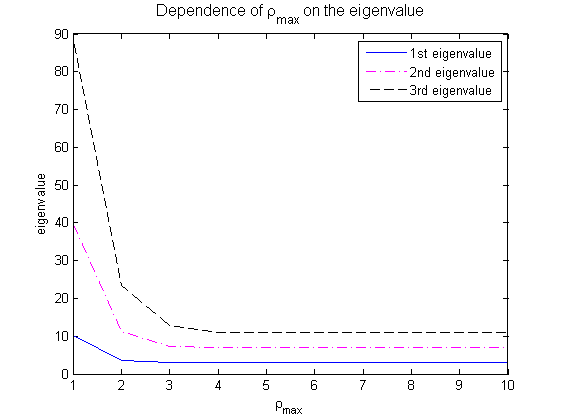
\includegraphics[width=0.75\textwidth]{Figures/rho_maxOnEigenvalue.png}
	\caption{Awesome caption}
	\label{fig:DependenceOnEigenvalue1}
\end{figure}
From the figure that if $\rho_{max} < 3$ the eigenvalues are varying dramatically.
This happens due to neglection ?? of strongly contributing parts of the eigenfunction. 
\fxnote{is this ok??}
\fxnote{comment on the flat part!!}
The $\rho_{max}$ that, with $n=100$, gives the most accurate result for all three of the first eigenvalues is $\rho_{max} = 5$. 
Since this $\rho_{max}$ gives the most accurate result for a relatively small $n$, this is chosen as the optimal $\rho_{max}$ in this and the following sections for this specific problem. 

With this $\rho_{max}$, we wish to find the number of $n$ that gives the first three eigenvalues with four leading digits. 
This optimal $n$ is found by steady increment of $n$, as seen in \fxnote{figref below}.
\begin{figure}[H]
	\centering
	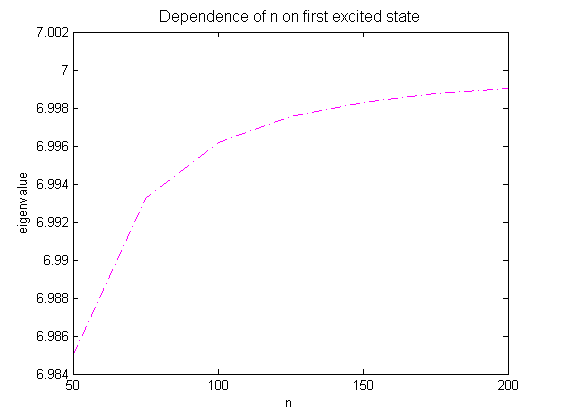
\includegraphics[width=0.75\textwidth]{Figures/MatrixSizeOnEigenvalue_2state.png}
	\caption{Awesome caption}
	\label{fig:DependenceOnEigenvalue2}
\end{figure}
The eigenvalue of the first exited is seen to be asymptotic to the analytical solution $\lambda_1 = 7$, and at a matrix size of $n=200$,  the eigenvalue of the first exited state has the numerical solution $6.99904$. 
This yields an accuracy up to four leading digits, which is also found to be the case for the ground state and the third eigenstate.
Hence, the optimal $\rho_{max}$ and $n$ is $5$ and $200$, respectively. 

	\subsection{Computation Time Compared to Alternative Algorithm}
\label{subsec:CompTime}
When calculating the time needed for the Jacobi rotation algorithm described in \fxnote{ref to section} to solve the eigenvalue problem with a matrix $\v{A}$ of dimensionality $200 \times 200$, $\rho_{max} = 5$, and $\epsilon = 10^{-8}$ the elapse time if found to be 17 sec.
\fxnote{ref to results} 
%using specified statements in c++
This is a much greater value than the elapsed time for solving the same eigenvalue problem using the Armadillo function 
\textit{eig\_sym} 
for the same $\epsilon = 10^{-8}$, since the Armadillo function has a displayed computational time of 0 sec (the computational time is of course not 0 sec, but the precision of the displayed time is so low that the number is displayed as 0). 
It is hence clear that the computed Jacobi algorithm consumes more time than the precomputed Armadillo function and as we increases the size of the matrix the elapsed time to get the solution also increases. 
This makes Jacobi rotation algorithm less efficient.

The following figures show the relation between the number of steps $n$ and the number of iterations of the while loop in the Jacobi algorithm computed for this project with the same $\rho_{max}$ and $\epsilon$ as described in the section above.
\begin{figure}[H]
\centering
\begin{minipage}{.5\textwidth}
  \centering
  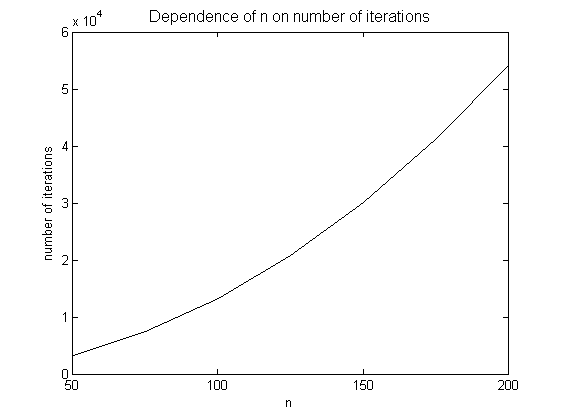
\includegraphics[width=1\linewidth]{figures/NumberOfIterations.png}
\end{minipage}%
\begin{minipage}{.5\textwidth}
  \centering
  \includegraphics[width=1\linewidth]{figures/NumberOfIterationsloglog.png}
\end{minipage}
\caption{The number of iterations of the while loop in the computed Jacobi method as a function of the number of steps $n$ plotted in both a normal graph and as a log-log plot. From the log-log plot it is evident that the number of iterations in the while loop is proportional to $n^2$, since the slope of the log-log plot is found to equal $2$.}
\label{fig:DependenceOnNumberOfIterations1}
\end{figure}
In the log-log plot, the relation is shown as a straight line with a slope of approximately $2$, which is calculated directly from the data for $n=100$ and $n=200$.
This yield that the number of iterations increases as the number of steps squared (that is, $n^2$), and hence an increment of $n$ has a great impact on the number of iteration. 
\fxnote{ikke sandt?}
E.g. with $n=100$ the number of iterations for the while loop in the Jacobi method is $13,200$, whilst when $n$ is doubled to $200$, the function runs through the while loop 54,071 times before the requirement of $max(a_{kl}^2) > \epsilon$ in \matref{eq:maxa} is fulfilled. 

The slowness of the Jacobi algorithm has the effect that it cannot be run for too large matrices, and hence there is a significant limit for how small the step length $h$ can be made, and ultimately a limit to the precision of the algorithm.  

It is, however, evident that the Jacobi method implemented in this project can be improved for solving the specific eigenvalue problem described by \matref{eq:NatureOfTheProblem5} and \eqref{eq:NatureOfTheProblem6} by taking into account that the matrix $\v{A}$ is tridiagonal and has constant values in the entrances adjacent to the diagonal.
\fxnote{reference ??} 
However, this improvement of the algorithm is not in the scope of this project.
	
\newpage 

\section{New potential and repulsive Coulomb interaction}

Until now the considered potential has been described by $\rho^2$ for one particle. When introducing another particle the potential is changed so the new potential is given by \matref{eq:Newpotential}, where $\omega$ is an oscillator frequency and $\frac{1}{\rho}$ is a repulsive Coulomb potential.
\begin{equation}
V_{\rho} = \omega^2\rho^2 + \frac{1}{\rho}
\label{eq:Newpotential}
\end{equation}

First considering the case without a repulsive Coulumb interaction. The aim is finding a value of $\rho_{max}$ so that the eigenvalues are considered stable.  
%----------------------------------
\begin{wraptable}{r}{5.0cm}
\caption{Table for finding best $\rho_{max}$ looking at the 1st eigenvalue} 
\label{tab:rhomax}
\phantom{.}
\begin{tabular}{|c|c|c|}
\hline
$\rho_{max}$ & N & 1st eigenvalue \\
\hline 
1 & 10 & 9.80273 \\
2 & 20 & 2.46292 \\
3 & 30 & 1.09594 \\
4 & 40 & 0.617001 \\
\vdots & \vdots & \vdots \\
9 & 90 & 0.124119\\
10 & 100 & 0.101504 \\
10.1 & 101 & 0.0996154 \\
11 & 110 & 0.0849622 \\
\hline

\end{tabular}

\end{wraptable}
%------------------------------------
For this to be stable the change should be small, so $\rho_{max} = 10$ and the change is about 0.02 between the surrounding steps. Also the change between 10 and 10.1 is about 0.002 so small changes in $\rho_{max} $ doesn't give big changes. Also the relation between $\rho_{max}$ and n is kept constant so that h is constant. Running for different values of $\rho_{max}$ with the ratio gives \tabref{tab:rhomax}, which shows that when $\rho_{max} $ is 10 the results are stable for the 1st eigenvalue. 


The Eigenvectors are used for determining the wave function, and in this case they are used squared so they show the probability density of the distance $\rho$ between the two electrons. Which gives the most probable distance between the particles,the distance $\rho = (\frac{1}{\alpha})r$ where $\alpha = (\frac{\hbar^2}{mk})^{1/4}$ is the Bohr radius. This is described in \secref{sec:NatureOfTheProblem}. And only the ground state is considered. Plotting the distance as a function of $\rho$ for different values of the frequency $\omega_r$, \figref{fig:ProbFuncOmegaWithout} shows that for a higher frequency $\omega_r$ the distance between the particles are bigger and the spread in area which the particle can be in is also more stretched out. 

\begin{figure}[H]
	\centering
	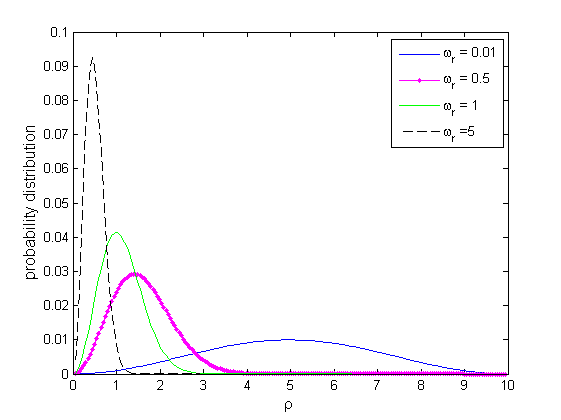
\includegraphics[width=0.75\textwidth]{Figures/2particles_without.png}
	\caption{The probability density as a function of distance $\rho$ without repulsive Coulomb interaction. Where $\rho_{min} = 0$, $\rho_{max} = 10$ and $n = 200$  }
	\label{fig:ProbFuncOmegaWithout}
\end{figure}

When adding a repulsive Coulomb potential $\frac{1}{\rho}$ to the potential $V(\rho )$ in \figref{fig:ProbFuncOmega} the probability density is pushed to a longer distance, although it might be a bit difficult to see in \figref{fig:ProbFuncOmega} and \figref{fig:ProbFuncOmegaWithout}. Physically it makes sense that the repulsive Coulomb interaction should increase the distance between the electrons as it gives a greater contribution when the electrons are close. The choice of $\rho$ is good because most of the probability distribution is inside the distance $\rho$. Also if there is no repulsive Coulomb interaction and the frequency $\omega = 1$ then the system acts as in the one particle case, and the choice of $\rho_{max} = 5$ there includes  most of the particle distributions. 

\begin{figure}[H]
	\centering
	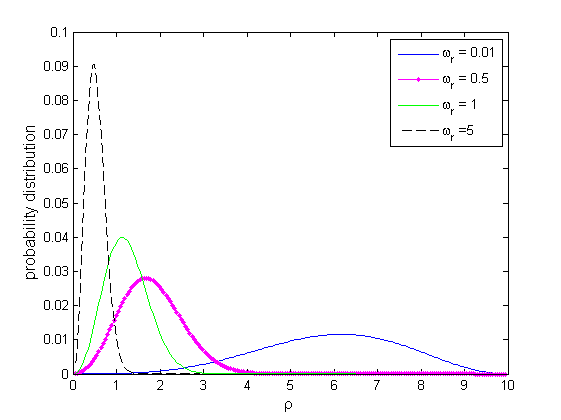
\includegraphics[width=0.75\textwidth]{Figures/ProbFuncOmega.png}
	\caption{The probability density as a function of distance $\rho$ with a repulsive Coulomb interaction. Where $\rho_{min} = 0$, $\rho_{max} = 10$ and $n = 200$}
	\label{fig:ProbFuncOmega}
\end{figure}






	\chapter{Conclusion}
Conclude.... conclude.... conclude....
 


	% ¤¤ LITTERATURLISTE: SKAL VÆRE SIDST ¤¤
		\bibliographystyle{ieeetr}
		\bibliography{Bibtex/litteratur}

% ¤¤ BILAG: SKAL VÆRE ALLERSIDST ¤¤
	\appendix
	\chapter{MatLab code for smt....}
\label{app:MatLabSolution}
This is how, we write MatLab code in the report
\lstset{language=Matlab}
\begin{lstlisting}
close all
clear all
clc
%I am a comment

filename = 'Results.xlsx';
sheet = 4;
xlRange = 'B3:C12';

[v,T,vT] = xlsread(filename, sheet, xlRange);
x10=v(:,1);y10=v(:,2);

figure
plot(??)
legend(??)

xlim([??])
ylim([??])

title(??)
xlabel('x')
ylabel('y')
\end{lstlisting}

	
\end{document}